\section{Theorie}

\subsection{CBCast Algorithmus}

In einem Netzwerk laufen verschiedene Prozesse auf verschiedenen Knoten und teilen sich keinen Speicherplatz. Die Interaktion zwischen den verschiedenen Prozessen läuft soweit ausschließlich über die Weitergabe von Nachrichten und kein Prozess kennt das Verhalten anderer Prozesse \cite{CBCAST_1}. Der \textit{CBCast} (Chain-Based Broadcast) Algorithmus ist ein Algorithmus der im Bereich der verteilten Systeme zum Einsatz kommt und eine Lösung für genau diese Prozessinteraktion implementiert. Genutzt wie zum Beispiel vom ISIS Projekt \cite{isis_project} hat er sich in der Vergangenheit bereits mehrfach renommiert.

\begin{figure}[htbp]
\begin{center}
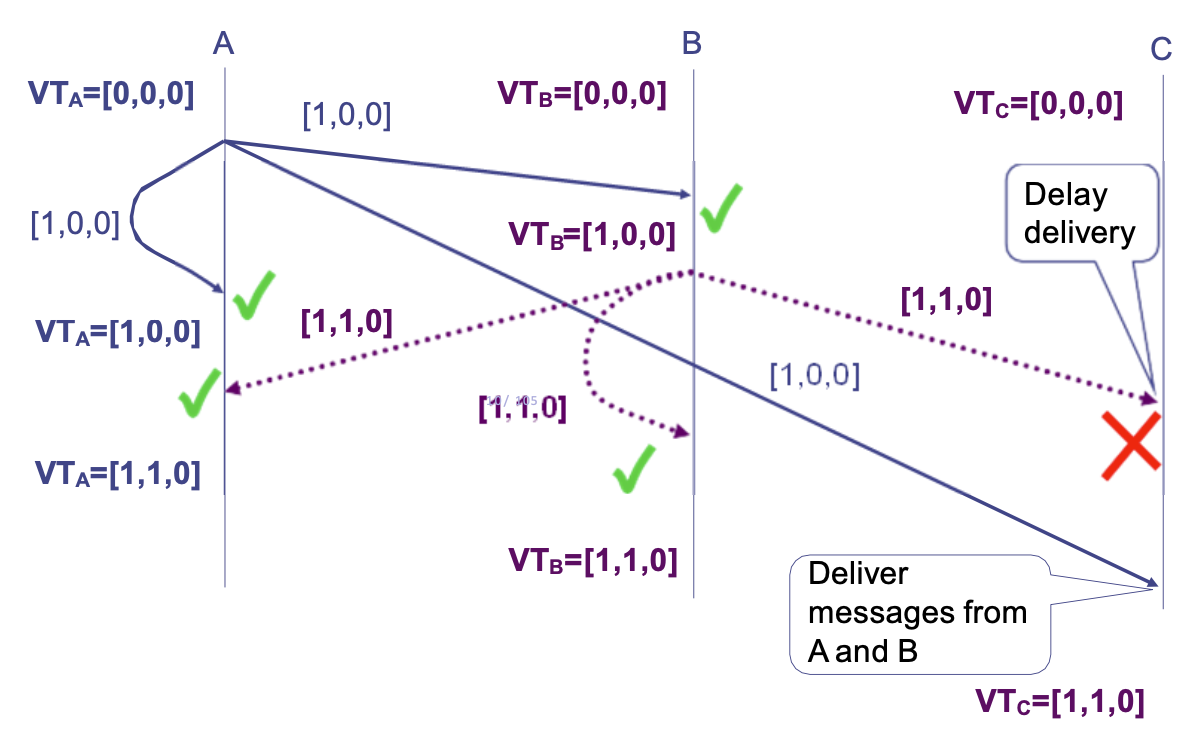
\includegraphics[scale=0.4]{Latex/Bilder/cbcast_1.png}
\caption{\label{fig:cbcastFunction} CBCAST \cite{Aufgabenstellung}} 
\end{center}
\end{figure}

In Abb. \ref{fig:cbcastFunction} zu sehen ist ein beispielhafter Ablauf des \textit{CBCASTs} mit drei Prozessen \textit{A}, \textit{B} und \textit{C}. VT zeigt die Vektoruhren der jeweiligen Prozesse. Hier wird der eigene Zeitstempel und der der anderen Prozesse individuell gespeichert. Durch diese Uhr können die Prozesse trotz fehlendem geteilten Speicherplatz erkennen, ob sie mit den anderen Prozessen synchronisiert sind.\\
Im ersten Schritt verschickt \textit{A} eine Nachricht an alle Teilnehmer im Netzwerk. Angehängt wird die eigene Vektoruhr - nun mit \textit{A} = 1 erhöht, da dieser Prozess die Nachricht verschickt hat. Wichtig hierbei ist, dass der sendende Prozess die Nachricht immer zusätzlich an sich selber schickt, um eine sichere Synchronisation sicherstellen zu können. In Abb. \ref{fig:cbcastFunction} empfangen Prozess \textit{A} und \textit{B} nun die von \textit{A} gesendete Nachricht. Die Vektoruhren werden verglichen und da jeweils nur ein Zeiger um 1 erhöht wurde, nehmen die Prozesse die gesendete Nachricht an. Nachdem \textit{B} die Nachricht von \textit{A} empfangen hat, schickt auch dieser Prozess eine Nachricht an alle Teilnehmer. \textit{A} und \textit{B} können diese empfangen. Beim Vergleichen der Vektoruhr von \textit{C} und der von \textit{B} mitgeschickten ist aber nun eine zu große Differenz. Zwei Zeiger sind jeweils um 1 erhöht, da \textit{B} bereits die Nachricht von \textit{A} empfangen hat. Bei \textit{C} fehlt diese noch, deshalb blockiert \textit{C}. Die Nachricht von \textit{A} welche daraufhin eintrifft nimmt \textit{C} dann an.\\
Die Zeiger in den Vektoruhren sind in vielen Implementierungen Zeitstempel der zuletzt empfangenen Nachricht.

\subsection{Kommunikationseinheit}

Die Kommunikationseinheit ermöglicht es Prozessen, welche über einen \textit{Tower} mit anderen Prozessen kommunizieren, Nachrichten zu schicken und zu empfangen. Das Interface stellt hierbei verschiedene Funktionen zum blockierenden und nicht blockierenden Senden von Nachrichten. Jeder Prozess, welcher als Kommunikationseinheit gestartet wird, empfängt bei korrekter Implementierung automatisch Nachrichten.

\subsubsection{Holdback Queue}

Beim Empfangen einer Nachricht, wird diese zuerst in eine \textit{Holdbackqueue} sortiert. Die \textit{Holdbackqueue} ist eine \textit{Priorityqueue} und enthält alle Nachrichten, die nicht ausgeliefert werden dürfen. Sortiert wird anhand der, der Nachricht angehängten, Vektoruhr.
\\Ob Nachrichten auslieferbar sind und die Queue verlassen dürfen oder ob Nachrichten aus der Queue gelöscht werden müssen, wird geprüft, wenn neue Nachrichten der Queue hinzugefügt werden. Falls es zu einem Stillstand im System kommt läuft zusätzlich ein Intervall-Timer, welcher die Auslieferbarkeitsprüfung regelmäßig aufruft.
\\Aus der Queue gelöscht werden, müssen Nachrichten welche %TODO

\subsubsection{Delivery Queue}

Die \textit{Deliveryqueue} ist die zweite Queue eines Kommunikationsprozesses. Sie enthält alle auslieferbaren Nachrichten und hat eine eigene Vektoruhr. Diese Vektoruhr wird synchronisiert mit jeder Vektoruhr einer, in der \textit{Deliveryqueue} neu hinzugefügten, Nachricht. 

\subsection{Ungeordneter Multicast}

Ein Multicast verteilt Nachrichten an Teilnehmer in einem Netzwerk. Der Unterschied zum Broadcast besteht darin, dass beim Broadcast Inhalte verbreitet werden, die – mit geeigneter Empfangsausrüstung – jeder ansehen kann, wohingegen beim Multicast vorher eine Anmeldung beim Sender erforderlich ist \cite{wiki:Multicast}.\\
Der TowerCBC (siehe Abb. \ref{fig:towerCBC}) übernimmt in dieser Ausarbeitung die Aufgabe des ungeordneten Multicasts. Ungeordnet ist dieser, weil die Nachrichten nicht in der Reihenfolge weitergegeben werden, in der sich die jeweiligen Teilnehmer/Prozesse beim TowerCBC registriert haben.

\begin{figure}[htbp]
\begin{center}
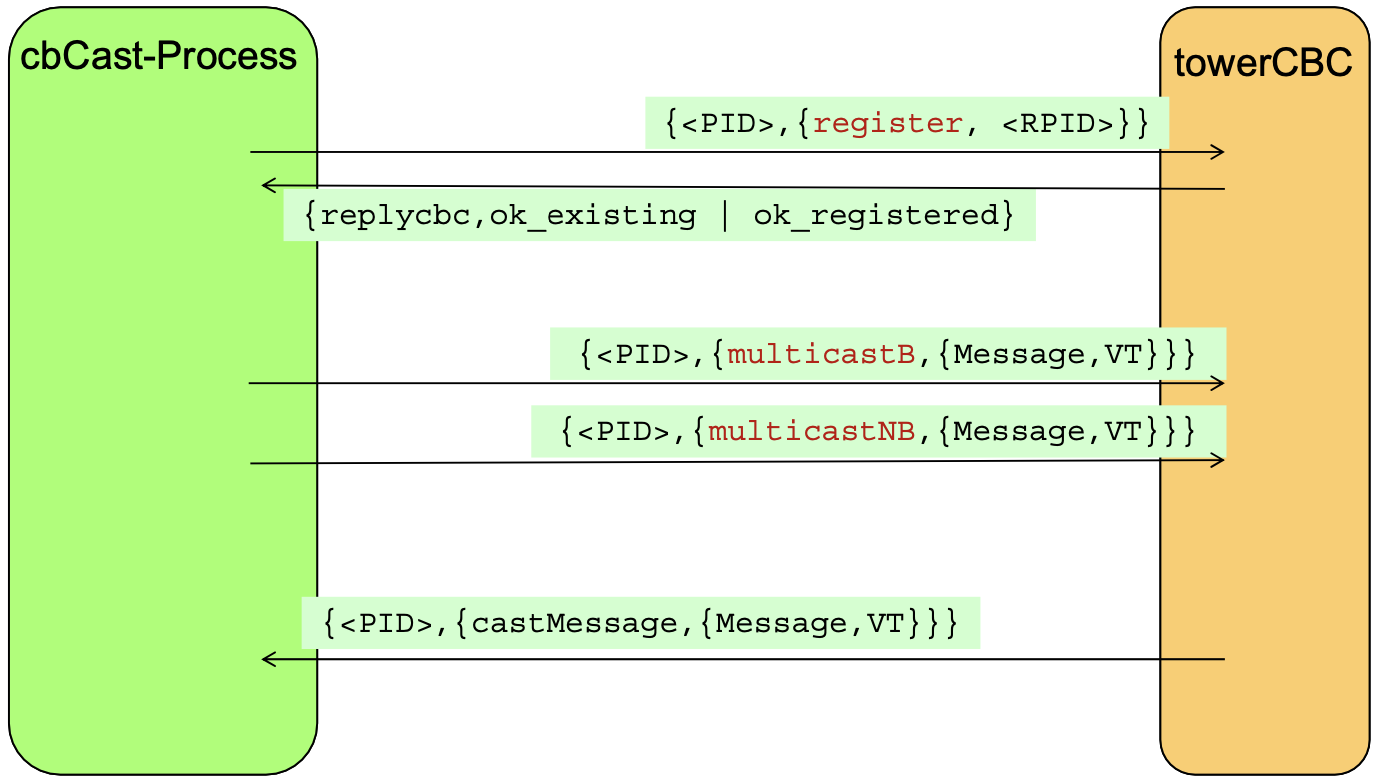
\includegraphics[scale=0.4]{Latex/Bilder/towerCBC_1.png}
\caption{\label{fig:towerCBC} ungeordneter Multicast \cite{Aufgabenstellung}} 
\end{center}
\end{figure}

In Abb. \ref{fig:towerCBC} ist eine abstrakte Kommunikation eines Prozesses mit dem Multicast dargestellt. Über \textit{register} meldet sich der \textit{cbCast-Prozess} beim \textit{towerCBC} an. Dieser bestätigt die Anmeldung. Über \textit{multicastB (blockierend)} oder \textit{multicastNB (nicht blockierend)} kann der Prozess nun Nachrichten über den Multicast an alle Teilnehmer im Netzwerk schicken. Der Multicast wieder kann mit \textit{castMessage} Nachrichten an die Teilnehmer schicken.

